\chapter{Facial Keypoints Detection}
\label{cha:Facial Keypoints Detection}

\section{Ausgangssituation}

Gesichtserkennung spielt im 21. Jahrhundert eine immer größer werdende Rolle. 
So existieren Herausforderungen mit den Schlüsselpunkten im Gesicht eines Menschen, welche wieder für Gesichtserkennungen verwendet werden können. 
Im Gesicht eines Menschen wird zum Beispiel die Iris in beiden Augen als Schlüsselpunkt definiert, aber auch die Nasenspitze und die Mundwinkel sowie weitere.
Diese Schlüsselpunkte variieren sehr stark von einem Individuum zum Nächsten, jedes Individuum hat eine Menge an Variationen. 
So spielt hier die Größe, die Position, die Neigung sowie die Beleuchtung eine Rolle und erzeugt eine fast unendliche Menge an Möglichkeiten. 
Mit Computer Vision konnten sehr viele Verbesserungen in diesem Bereich erzielt werden, wobei noch sehr viel Raum für Forschung und Verbesserungen bleibt. \newline

\noindent
Die Aufgabenstellung wird auf der Online-Plattform Kaggle \footnote{Kaggle: Facial Keypoints Detection \url{https://www.kaggle.com/c/facial-keypoints-detection}} gehostet, wo auch die Trainings- und Testdaten zur Verfügung gestellt werden. 
Diese Aufgabe war im Jahr 2016 eine Herausforderung, an der sich jeder beteiligen konnte, um den ersten Platz zu erreichen. 
Das Ziel für jeden Teilnehmer war es ein System zu entwickeln, welches mit den Trainingsdaten trainiert wird.
Im Anschluss sollte dieses System dann mit den Testdaten getestet werden. 
Das Ergebnis musste im Anschluss eingereicht werden, welches dann überprüft und bewertet wurde. 

\section{Vorbereitung}

Die Daten, die zur Verfügung gestellt werden, sind auf mehreren Dateien aufgeteilt. 
In diesem Fall beinhaltet die Datei mit den Trainingsdaten die meisten Daten. 
Sie beinhaltet die Bilder der Gesichter, sowie die Koordinaten der Schlüsselpunkte, gespeichert in einer CSV-Notation.
%Im gesamten Gesicht gibt es 15 Schlüsselpunkte welche hier berücksichtigt werden. 
Im gesamten Gesicht werden in diesem Beispiel 15 Schlüsselpunkte berücksichtigt. 
In der Auflistung \ref{fig:15keypoints} sind die Bezeichnungen der Spalten mit den Werten ersichtlich, wobei zu jeder Bezeichnung ein \glqq X\grqq und ein \glqq Y\grqq existiert.
Ein Beispiel dazu ist in der Auflistung \ref{fig:ausgangsdatenRoh} zu finden.
\begin{lstlisting}[caption={$15$ Schlüsselpunkte im Gesicht eines Menschen},label=fig:15keypoints,captionpos=b,language=Python]
left_eye_center, right_eye_center, 
left_eye_inner_corner, left_eye_outer_corner, right_eyee_inner_corner, right_eye_outer_corner, 
left_eyebrow_inner_end, left_eyebrow_outer_end, right_eyebrow_inner_end, right_eyebrow_outer_end, 
nose_tip, 
mouth_left_corner, mouth_right_corner, 
mouth_center_top_lip, mouth_center_bottom_lip
\end{lstlisting}
Jeder diese Schlüsselpunkte besteht aus einer X und einer Y Koordinate. 
Diese Datei besitzt zusätzlich in der $31.$ Spalte das Bild mit dem dazugehörigen Gesicht.
Das Bild ist encodiert abgelegt und besteht aus $96 * 96$ Werten. 
In diesem Sinne stehen nur Bilder in Graustufen zur Verfügung mit einer Auflösung von $96 * 96$ Pixel und einer Farbtiefe von $[0, 255]$, wie in der Abbildung \ref{fig:ausgangsdaten} zu erkennen ist. 
Für diese Aufgabe werden im Grunde auch nur die Konturen benötigt, was somit den einen Farbkanal erklärt, aber auch die Aufgabe schwieriger macht, denn mehrere Farbkanäle könnten mit Filter bearbeitet werden und so noch weitere Konturen hervorheben. 
\begin{figure}
	\centering
	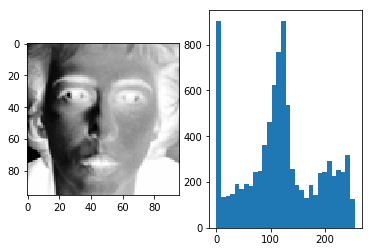
\includegraphics[scale=0.75]{images/ausgangsDaten.png}
	\caption{Ein Gesicht aus dem Datenbestand mit der Verteilung der Graustufenwerten}
	\label{fig:ausgangsdaten}
\end{figure}
	\begin{lstlisting}[caption={Ein gesamter Datensatz aus den Trainingsdaten mit den X und Y Werten pro Schlüsselpunkt},label=fig:ausgangsdatenRoh,captionpos=b,language=Python]
# left\_eye\_center, right\_eye\_center
66.0335639098,39.0022736842,30.2270075188,36.4216781955
# left\_eye\_inner\_corner, left\_eye\_outer\_corner
59.582075188,39.6474225564,73.1303458647,39.9699969925
# right\_eye\_inner\_corner, right\_eye\_outer\_corner
36.3565714286,37.3894015038,23.4528721805,37.3894015038
# left\_eyebrow\_inner\_end, left\_eyebrow\_outer\_end
56.9532631579,29.0336481203,80.2271278195,32.2281383459
# right\_eyebrow\_inner\_end, right\_eyebrow\_outer\_end
40.2276090226,29.0023218045,16.3563789474,29.6474706767
# nose\_tip
44.4205714286,57.0668030075
# mouth\_left\_corner, mouth\_right\_corner
61.1953082707,79.9701654135,28.6144962406,77.3889924812
# mouth\_center\_top\_lip, mouth\_center\_bottom\_lip
43.3126015038,72.9354586466,43.1307067669,84.4857744361
# image
238 236 237 238 240 240 239 241 241 243 240 239 231 212 ...
\end{lstlisting}

\subsection{Daten vorbereiten und normalisieren}

Zu Beginn diese Daten müssen vorbereitet und normalisiert werden. 
Um die Problemgröße zu verringern, empfiehlt es sich, die Aufgabe auf mehrere Netzwerke aufzuteilen. 
Dies hat einen zusätzlichen Grund, da die Trainingsdaten nicht komplett sind und somit nicht zu allen Bildern alle 15 Schlüsselpunkte vorhanden sind. 
Sollte dies ignoriert werden, würde sich die Anzahl der zur Verfügung stehenden Datensätze von $7049$ auf $2140$ reduzieren. 
Ein weiterer Grund für die Auftrennung der Problemstellung ist, dass Aufgaben leichter verteilt werden können und die Netzwerke noch genauer angepasst werden könnten. \newline

\noindent
Unter der Zuname von Pandas\footnote{Pandas: Python Data Analysis Library \url{http://pandas.pydata.org/}} und NumPy\footnote{NumPy: Scientific Computing \url{http://www.numpy.org/}} besteht die Möglichkeit, sehr einfach und effizient auf die Datensätze zuzugreifen und diese zu verwenden. 
Wie im Codebeispiel \ref{fig:datenLesenEinschränken} ersichtlich ist, werden die Daten mit Hilfe von Pandas geladen und unter Zunahme von NumPy normalisiert und neu strukturiert. 
\begin{lstlisting}[caption={Daten einlesen und einschränken},label=fig:datenLesenEinschränken,captionpos=b,language=Python]
import pandas as pd
import numpy as np

# konstanten Definition
IMAGE_SIZE = 96

# Daten einlesen
df = pd.read_csv('~/training.csv')

# Bilder um konvertieren in eine List von Zahlen
df['Image'] = df['Image'].apply(lambda im: np.fromstring(im, sep=' '))

# die Aktuell benötigten Spalten herausnehmen
df = df[['left_eye_center', 'right_eye_center', 'Image']]

# entfernen unvollständiger Datensätze
# Verringerung der Datensätze von 7049 auf 7033
df = df.dropna()

# normalisieren der Bilder in einen Wertebereich von [0, 1] 
# und überführen in eine 96 mal 96 Matrix
# Variable X beinhaltet alle Bilder des Datensatzes welche Vollständig sind
X = np.vstack(df['Image']) / 255.
X = X.reshape(-1, IMAGE_SIZE, IMAGE_SIZE, 1)

# explizites definieren des Datentyps für die Werte der Bilder
X = X.astype(np.float32)

# narmalisieren der Y Koordinaten in einen Wertebereich von [0, 1]
# Variable Y beinhaltet die Labels zu allen Bildern
Y = df[df.columns[:-1]].values
Y = Y / 96.0
\end{lstlisting}

\subsection{Evaluations- und Errorfunktion}

Die Ergebnisse des Netzwerkes müssen immer verglichen und validiert werden. 
In diesem Beispiel handelt es sich nicht um eine Klassifizierungsaufgabe, sondern um eine Regressionsproblemstellung. 
Deshalb kann nicht einfach eine 'Cross Entropy' Funktionen verwendet werden, um die Daten zu evaluieren und zu adaptieren. 
Aus diesem Grund muss dies manuell durchgeführt werden und selbst eine Berechnung aufgestellt werden, welche diese Werte liefert, damit diese einem Optimierer übergeben werden können. 
Der Verlust, beziehungsweise die Differenz zwischen Ergebnis des Netzwerkes und dem bekannten Ergebnis, kann durch eine Subtraktion sowie einer Quadrierung berechnet werden. 
Diese ist in der Gleichung \ref{eq:lossCalc} zu erkennen, wobei \textit{graph} eine Matrix (Tensor) an Ergebnissen ist, mit der Anzahl an Zeilen wie in der Konstante \textit{BATCH\_SIZE} definiert. 
Die Variable \textit{train\_labels\_node} beinhaltet die bekannten Ergebnisse zu Bildern mit denselben Dimensionen wie in der Matrix \textit{graph}. 
\textit{tf.subtract} führt eine Subtraktion auf jeden einzelnen Wert der beiden Matrizen aus, was auch dazu führt, dass diese dieselben Dimensionen haben müssen. 
\textit{tf.square} quadriert die berechneten Differenzen um negative Werte zu entfernen. 
Zum Abschluss werden alle Ergebnisse in der Ergebnismatrix mit \textit{tf.reduce\_sum} aufsummiert, was zu einem Skalar führt. 
Für diese konkrete Implementierung wurde als Optimierungsalgorithmus ein \textit{Adam}-Algorithmus \cite{DBLP:journals/corr/KingmaB14} verwendet. 
Um das Verlustergebnis für einen Leser lesbarer zu machen, muss der Verlustwert durch die Anzahl der Batchgröße dividiert werden, was die Differenz in einem Datensatz als Durchschnitt ergibt, ohne die Quadrierung zu berücksichtigen. 
Die gesamte Umsetzung ist im Codebeispiel \ref{fig:VerlustKonkreOpitimier} zu finden. 
\begin{equation}
	Verlust := \sum{(R - L)^2}
	\label{eq:lossCalc}
\end{equation}
\begin{lstlisting}[caption={Verlustberechnung, konkreter Opitimierungsalgorithmus, Genauigkeitsberechnung},label=fig:VerlustKonkreOpitimier,captionpos=b,language=Python]
import tensorflow as tf

# Konstanten Definition
BATCH_SIZE = 20

# Verlustberechnung
with tf.name_scope("loss"):
    # sollte sich im Laufe der Trainingsphasen an 0 annähern
    loss = tf.reduce_sum(
    			tf.square(
    				tf.subtract(graph, train_labels_node)))

# Auswahl eines konkreten Optimierungsalgorithmuses in der Kurzschreibweise
# mit einer Lernrate von 0.00001
with tf.name_scope("train"):
    train = tf.train.AdamOptimizer(learning_rate=1e-5).minimize(loss)
    
# Verlustwert durch die Anzahl der Bilder im Batch da diese 
# in der loss-Berechnung zusammen summiert werden
with tf.name_scope("accuracy"):    
    accuracy = loss / BATCH_SIZE
\end{lstlisting}
 
\section{Neuronale Ebenen vorbereiten}

Damit die Ebenen einfacher verwendet werden können, können diese als konfigurierbare Muster definiert werden. 
Dadurch wird erzielt, dass gleiche Ebenen im visualisierten Graphen dieselbe Farbe besitzen und zum anderen alle Inhalte darin zusammengefasst werden. 
Im Grunde existieren zwei verschiedene Haupttypen an Ebenen. 
Zum einen die Convolutional-Ebenen und zum anderen die Vollvernetzten-Ebenen. 
Wie im Code \ref{fig:ConvFc} ersichtlich ist, besitzen beide Hauptgruppen an Ebenen jeweils eine Datenquelle, beschrieben als \textit{x\_} und Gewichtungen und Biaseswerte. 
Die Bias-Werte werden dabei erst nach der Kernfunktion an das Ergebnis angefügt und somit erst in der Aktivierungsfunktion berücksichtigt. 
\begin{lstlisting}[caption={Definition der Convolutional- und Vollvernetzten-Ebenen},label=fig:ConvFc,captionpos=b,language=Python]
def conv_layer(x_, size_in, size_out, name="conv"):
    with tf.name_scope(name):
        weights = tf.Variable(tf.truncated_normal(
        						[3, 3, size_in, size_out], 
        						dtype=tf.float32, stddev=1e-1), 
							trainable=True, name='weights')
        conv = tf.nn.conv2d(x_, weights, [1, 1, 1, 1], padding='SAME')
        biases = tf.Variable(tf.constant(0.0, 
								shape=[size_out], dtype=tf.float32), 
                            trainable=True, name='biases')
        bias = tf.nn.bias_add(conv, biases)
        conv = tf.nn.relu(bias, name="act")

    maxPool = tf.nn.max_pool(conv, 
                             ksize=[1, 2, 2, 1],
                             strides=[1, 2, 2, 1],
                             padding='VALID')
    return conv

def fc_layer(x_, size_out, name="fc", act=None):
    with tf.name_scope(name):
        size_in = x_.get_shape()[1].value
        weights = tf.Variable(tf.truncated_normal([size_in, size_out], 
								dtype=tf.float32, stddev=1e-2), 
							trainable=True, name='weights')
        biases = tf.Variable(tf.constant(0.0, shape=[size_out], 
								dtype=tf.float32), 
							trainable=True, name='biases')
        mul = tf.nn.xw_plus_b(x_, weights, biases)
        
        if act is not None:
            mul = act(mul)
        return mul
\end{lstlisting}

\section{Neuronale Ebenen verknüpfen}

Diese Definitionen der Ebenen aus dem Codefragment \ref{fig:ConvFc} müssen im nächsten Schritt zu einem Netzwerk zusammengesetzt werden. 
Ein neuronales Netzwerk, welches relativ leichtgewichtig ist und diese Problematik relativ brauchbar lösen kann, ist im Grunde ein sehr vereinfachtes 'VGG16' Netzwerk\footcite{VGG16: https://arxiv.org/pdf/1409.1556.pdf}. 
Für diesen Fall besteht dieses aus $3$ Convolutional-Ebenen und $3$ Vollvernetzten-Ebenen, wie im Codefragment \ref{fig:buildGraph} zu sehen ist. 
Das originale VGG16 Netzwerk besitzt im Gegensatz zum aktuell verwendeten, $5$ Convolutional-Ebenen mit je $2$ integrierten Convolutional-Ebenen mit denselben Dimensionen, die Hauptebenen $3$ bis $5$ zusätzlich eine $3$ Convolutional-Ebene. 
Die letzte Ebene der Vollvernetzten-Ebenen wird dabei ohne Aktivierungsfunktion ausgeführt, um die Roh-Ergebnisse zu bekommen. 
Im aktuellen Fall werden für die $2$ Iris-Positionen im Gesicht $4$ Ergebnisse benötigt. 
An diesem Beispiel lässt sich erkennen, dass hier Variablen wiederverwendet werden, dies ist durch Python möglich und durch die Beschreibung des Graphen, welcher im Hintergrund aufgebaut und verbunden wird. 
\begin{lstlisting}[caption={Modelldefinition des Graphen},label=fig:buildGraph,captionpos=b,language=Python]
def model(data):
    net = conv_layer(data, 1, 32, "conv1")
    net = conv_layer(net, 32, 64, "conv2")
    net = conv_layer(net, 64, 128, "conv3")

    # Transformieren in eine flache Struktur
    dims = net.get_shape()[1:]
    k = dims.num_elements()
    with tf.name_scope('flatten'):
        net = tf.reshape(net, [-1, k])
    
    net = fc_layer(net, 256, "fc1", tf.nn.relu)    
    net = fc_layer(net, 256, "fc2", tf.nn.relu)
    net = fc_layer(net, 4, "fc3")
    
    return net
    
# Definition der Platzhalter für die Datenübergabe
train_data_node = tf.placeholder(tf.float32, 
						shape=(BATCH_SIZE, IMAGE_SIZE, IMAGE_SIZE, 1))
train_labels_node = tf.placeholder(tf.float32, 
						shape=(BATCH_SIZE, 4))

# erstellen eines Graphen mit dem definierten Model
graph = model(train_data_node)
\end{lstlisting}

\section{Trainieren}

Um das erzeugte Netzwerk aus \ref{fig:buildGraph} verwenden und trainieren zu können, muss dieses zuerst initialisiert werden. 
Wie im Code \ref{fig:initRun} zu erkennen ist, wird eine globale Initialisierung verwendet, welche alle Konstanten und Variablen der aktuellen Umgebung initialisiert. 
In der For-Schleife werden fast alle Datensätze einmal durch den Graphen gesendet und entweder zum Trainieren oder Evaluieren verarbeitet. 
Der Session wird in der \textit{Run}-Methode eine Liste an Punkten des Graphen mitgegeben, welche evaluiert werden sollen. 
In der Trainingsphase ist dies der Optimierungsendpunkt und in der Evaluierungsphase die Punkte \textit{accuracy} und \textit{graph}. 
\textit{accuracy}, damit ein vergleichbarer Wert zur Verfügung steht, an welchem der Lernfortschritt erkennbar ist und der Hauptendpunkt des Graphen selbst, damit die Ergebnisse direkt in Bilder gezeichnet werden können. 
Dies ermöglicht eine visuelle Verifikation durch einen Supervisor. 
Dieses Codefragment ergibt eine sogenannte Epoche, in der alle Datensätze einmal vom Netzwerk verarbeitet werden. 
\begin{lstlisting}[caption={Initialisierung des Graphen und Durchführen einer Epoche},label=fig:initRun,captionpos=b,language=Python]
# erstellen einer Session
sess = tf.Session()

# erstellen einer globalen Initialisierungsroutine
init_op = tf.global_variables_initializer()
# initialisieren aller Konstanten und Variablen
sess.run(init_op)

# durchlaufen aller Datensätze -> 1 Epoche
runing = train_data.shape[0] // BATCH_SIZE
for i in range(runing):
    offset = i * BATCH_SIZE
    
    # laden eines Datenbatches aus den Datensätzen
    batch_data = train_data[offset:(offset + BATCH_SIZE), ...]
    batch_labels = train_labels[offset:(offset + BATCH_SIZE)]
    
    # ersetzen der Platzhalter durch die konkreten Daten
    feed = {train_data_node: batch_data, 
            train_labels_node: batch_labels}
     
    # ausführen des Graphen zur Evaluierung
    if i % 5 == 0:
        [train_accuracy, data] = sess.run([accuracy, graph], 
        								 feed_dict=feed)
        print data[0:4]
        print batch_labels[0:4]
        
        print i, train_accuracy
    # ausführen einer Trainingsiteration
    else:
        sess.run(train, feed_dict=feed)
\end{lstlisting}

\section{Validierungsergebnisse}

Durch längeres Trainieren kann sich das Netzwerk entwickeln und im Lauf der Epochen bessere Ergebnisse liefern. 
Dies führt natürlich auch zu der Möglichkeit, dass das Netzwerk beginnt, Muster zu speichern anstatt zu lernen, auch bekannt als Overfitting. 
In der Abbildung \ref{fig:runns} sind die Ergebniszustände am Ende der 100. Epoche sowie am Ende der 150. Epoche zu sehen. 
Im Gesamten kann festgestellt werden, dass das Netzwerk seine Arbeit relativ korrekt erledigt, wenn man die Größe und Dimension des Netzwerkes berücksichtigt. 
\begin{lstlisting}[caption={Ergebnisse am Ende der 100. Epoche und am Ende der 150. Epoche},label=fig:runns,captionpos=b,language=Python]
.... Epochen 100 ....
# Ist-Ergebnis 
[[ 0.66568404  0.38626809  0.35157766  0.4218266 ]
 [ 0.68138432  0.40295351  0.27889865  0.40295351]
 [ 0.676839    0.4047336   0.3197888   0.397911  ]
 [ 0.66469301  0.41260486  0.29902736  0.42368389]]
# Soll-Ergebnis
[[ 0.69634622  0.37385067  0.32604855  0.38231322]
 [ 0.70251364  0.34271669  0.32569841  0.3908942 ]
 [ 0.67929983  0.36809221  0.2629534   0.36637166]
 [ 0.71011567  0.39950868  0.3037816   0.3843804 ]]
# Trainingsgenauigkeit
0.0001787
.... Epochen 150 ....
# Ist-Ergebnis
[[ 0.6832875   0.381525    0.32855     0.40945625]
 [ 0.67460902  0.36388947  0.33187218  0.38741128]
 [ 0.68836184  0.38701776  0.29144079  0.38995789]
 [ 0.6741519   0.37355443  0.32906962  0.40749367]]
# Soll-Ergebnis
[[ 0.67965472  0.3785463   0.32667899  0.40375352]
 [ 0.67585701  0.35977855  0.33285627  0.38183641]
 [ 0.68490797  0.38329497  0.29059213  0.3844119 ]
 [ 0.67040122  0.3710691   0.32904905  0.40210161]]
# Trainingsgenauigkeit
5.38928e-05
\end{lstlisting}
Zum besseren Feststellen des Ergebnisses befindet sich in der Abbildung \ref{fig:resultPic} ein direkter Vergleich. 
Dabei wird der Istzustand durch blaue Punkte gekennzeichnet. 
\begin{figure}[ht!]
	\centering
	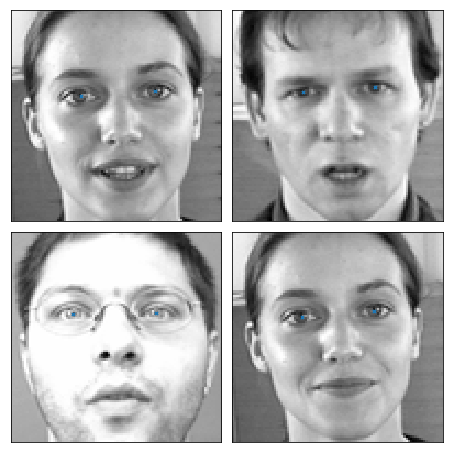
\includegraphics[scale=0.5]{images/normal.png}
	\caption{Ist-Visualisierung des Ergebnisses}
	\label{fig:resultPic}
\end{figure}

\section{Ergebnis}

In der Abbildung \ref{fig:lossDiag} sind die gesamten Trainingsergebnisse in Form der Verluste aufgezeichnet. 
Diese wiederum ergeben sich aus dem quadrierten Abstand zwischen Soll- und Ist-Punkt.
In diesem Fall nähert sich der Verlustwert der $0$-Grenze, trotzdem scheint es ein Probleme mit einigen Daten zugeben. 
Eine mögliche Interpretation wäre, dass die Lernrate mit '$1e-5$' noch zu hoch definiert wurde und sich das Netzwerk so zu schnell einem lokalen Minima genähert hat, obwohl es möglicherweise ein globales Minima gegeben hätte. 
Eine andere Möglichkeit wäre, dass die Datensätze Bilder beinhalten, in welchem das Gesicht nicht vollständig zu erkennen ist oder dass diese stärker rotiert sind. 
Sollte es nicht so viel Datensätze mit diesen Eigenheiten geben, so könnte dies ein weiterer Grund sein warum das Netzwerk springt. 
Dies bedeutet, dass ein nicht stabiler Zustand vorhanden ist und möglicherweise ein Rauschen in den Daten nicht ignoriert wurde sondern darauf reagiert wird.
In der Abbildung \ref{fig:lossDiag} lässt sich erkennen, dass die Sprünge nicht regelmäßig sind, was auf ein Mischen der Datensätze am Ende jeder Epoche zurückgeführt werden kann. 
\begin{figure}[ht!]
	\centering
	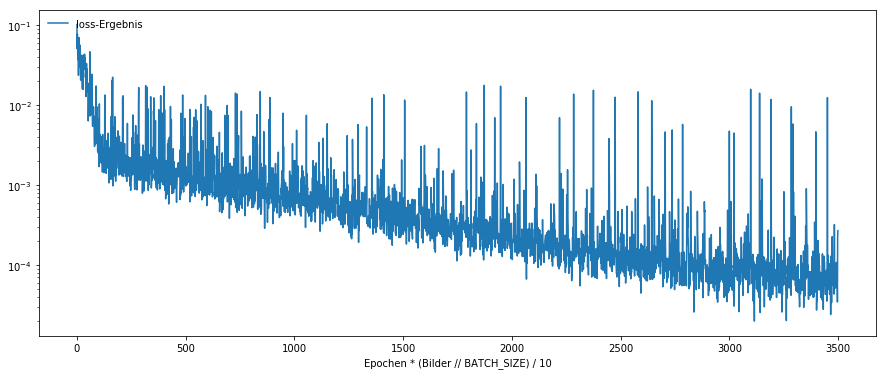
\includegraphics[scale=0.4]{images/loss-diagram-all-new.png}
	\caption{Trainings-Verlustergebnisse in 100 Epochen mit 350 Tests pro Epoche}
	\label{fig:lossDiag}
\end{figure} \phantom \newline

\noindent
Durch einen Test aller Datensätze und herausfinden des Besten und des Schlechtesten Ergebnisses, lässt sich feststellen warum das Netzwerk diverse Probleme mit Bildern besitzt. 
Im Konkreten beinhalten die Daten einige wenige dubiose Bilder. 
Ein Beispiel dazu befindet sich in der Abbildung \ref{fig:dubio}. 
Hier ist erkennbar, dass sich in den zwei oberen Bildern, mehrere Bilder auf einem WhiteBoard vorhanden sind. 
Zum Einen ist hier das Problem, dass sich hier mehr als ein Gesichter im Bild befindet und das Netzwerk nicht für so einen Fall ausgelegt und trainiert worden ist. 
Zum Anderen lässt sich erkennen, dass das Netzwerk hier ein anderes Bild bevorzugt, auf welchem ebenfalls Menschen abgebildet sind. 
Dies führt zu der Annahme, dass das Netzwerk sich hier nicht die Positionen durch das Trainieren gemerkt hat und dies als Rauschen wahrnimmt. 
Sowie sich an die sonst zentralisierten Gesichter orientiert und trotzdem versucht hier zwei Augen zu finden, welche mehr oder weniger nebeneinander liegen sollten. 
In den zwei unteren Bildern kann festgestellt werden, dass das Netzwerk akkuraten Ergebnisse liefert. 
\begin{figure}[ht!]
	\centering
	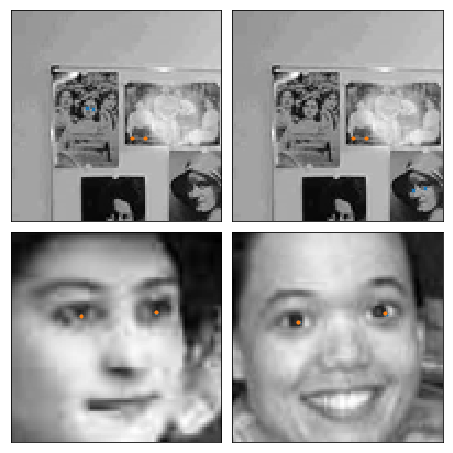
\includegraphics[scale=0.6]{images/Bad_2.png}
	\caption{Schlechtester Fall in der 150. Epoche; blauer Punkt = Soll-, roter Punkt = Ist-Wert}
	\label{fig:dubio}
\end{figure} \phantom \newline

\noindent
Im besten Fall erzielt das Netzwerk eine Abweichung von $5.1624589e-05$, was in der 150. Epoche als sehr positiv gewertet werden kann.
Das beste Ergebnis der 150. Epoche ist in der Abbildung \ref{fig:good} ersichtlich. 
An diesem Ergebnis lässt sich erkennen, dass das Netzwerk mehr oder weniger keine Probleme mit diversen Hautfarben und Kontrasten hat. 
Des Weiteren werden Brillen ignoriert und auch leichte Neigungen nach links und rechts stellen keine Schwierigkeit dar. 
\begin{figure}[ht!]
	\centering
	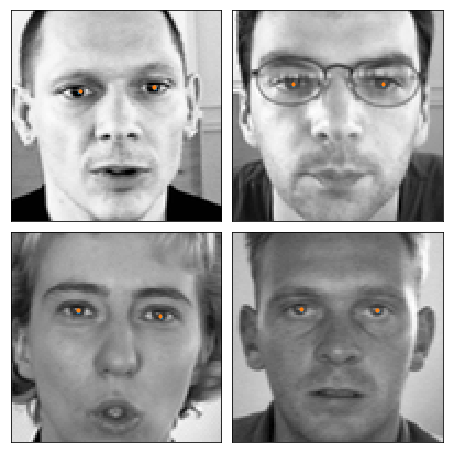
\includegraphics[scale=0.6]{images/Good_2.png}
	\caption{Bester Fall in der 150. Epoche; blauer Punkt = Soll-, roter Punkt = Ist-Wert}
	\label{fig:good}
\end{figure} \phantom \newline

\noindent
Im Langzeittest bis zu der 800. Epoche lässt sich feststellen, dass das Netzwerk noch genauer wird, wobei hier der zeitliche Aufwand für das Trainieren sehr viel Zeit beansprucht und zusätzlich das Problem des Overfittung akut werden könnte. 
In der Tabelle \ref{tab:time} sind zwei Systeme aufgeführt auf welchem das Netzwerk trainiert wurde, wo der Berechnungsvorteil der GPU deutlich ersichtlich ist. 
\begin{table}[htb]%[ht!]
\centering% NICHT \begin{center}
\begin{tabular}{c c c}
%\hline 
System & 1 Epoche & 100 Epochen \\ 
\hline 
Amazon EC2 Instanz, c3.8xlarge \\ Intel Xeon E5-2680 v2, 32 Kerne 60 GiB Ram \\ keine GPU & 466 & 46609 \\ 
\hline 
Dell Optiplex 790 \\ Intel Core 2 Duo CPU E8400, 2 Kerne, 8 GiB Ram \\ Nvidia TitanX, 12 GiB & 87 & 8700 \\ 
%\hline 
\end{tabular} 
\caption{Aufschlüsselung der ungefähr benötigten Berechnungszeiten für eine und 100 Epochen in Sekunden}
\label{tab:time}
\end{table} \phantom \newline

\noindent
Zur genaueren Feststellung der Funktionalität des Netzwerkes befindet sich in der Abbildung \ref{fig:meTest} ein Test mit einem noch komplett unbekannten Gesicht. 
Dieses wurde für diesen Test manuell aufgenommen und konvertiert sowie im Weiteren in das Netzwerk als Testdatensatz eingefügt. 
Wie zu erkennen ist, befindet sich das Netzwerk in der 150. Epoche bereits in einem Zustand, welcher als verwendbar einstuft werden kann. 
\begin{figure}[ht!]
	\centering
	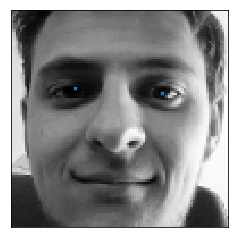
\includegraphics[scale=0.8]{images/me-test.png}
	\caption{Testaufnahme mit Ergebnis des Netzwerkes}
	\label{fig:meTest}
\end{figure}

\section{Graphenvisualisierung}

Der Graphen wurde in diesem Beispiel in ein Event-File serialisiert, dabei wurde aus Performanzgründen die Speicherung von Veränderungen in den Ebenen sowie anderer Skalar-Werten weggelassen. 
In der Abbildung \ref{fig:graphDig} ist der aktuelle Graph des Beispiels ersichtlich. 
Dieser beinhaltet die $3$ Convolutional-Ebenen, die Transformation in eine flache Struktur sowie die Vollvernetzten-Ebenen und den Optimizer sowie die Verlustberechnung. 
Im Gesamten lässt sich ein Graph erkennen, in welchem der Datenfluss am Ende beginnt und nach oben läuft. 
Am Rande der Abbildung befinden sich noch zwei zusätzliche Objekte, welche Verbindungen zu allen Objekten haben. 
Diese werden automatisch durch TensorFlow hinzugefügt und werden für die Ausführung benötigt. 
\begin{figure}[ht!]
	\centering
	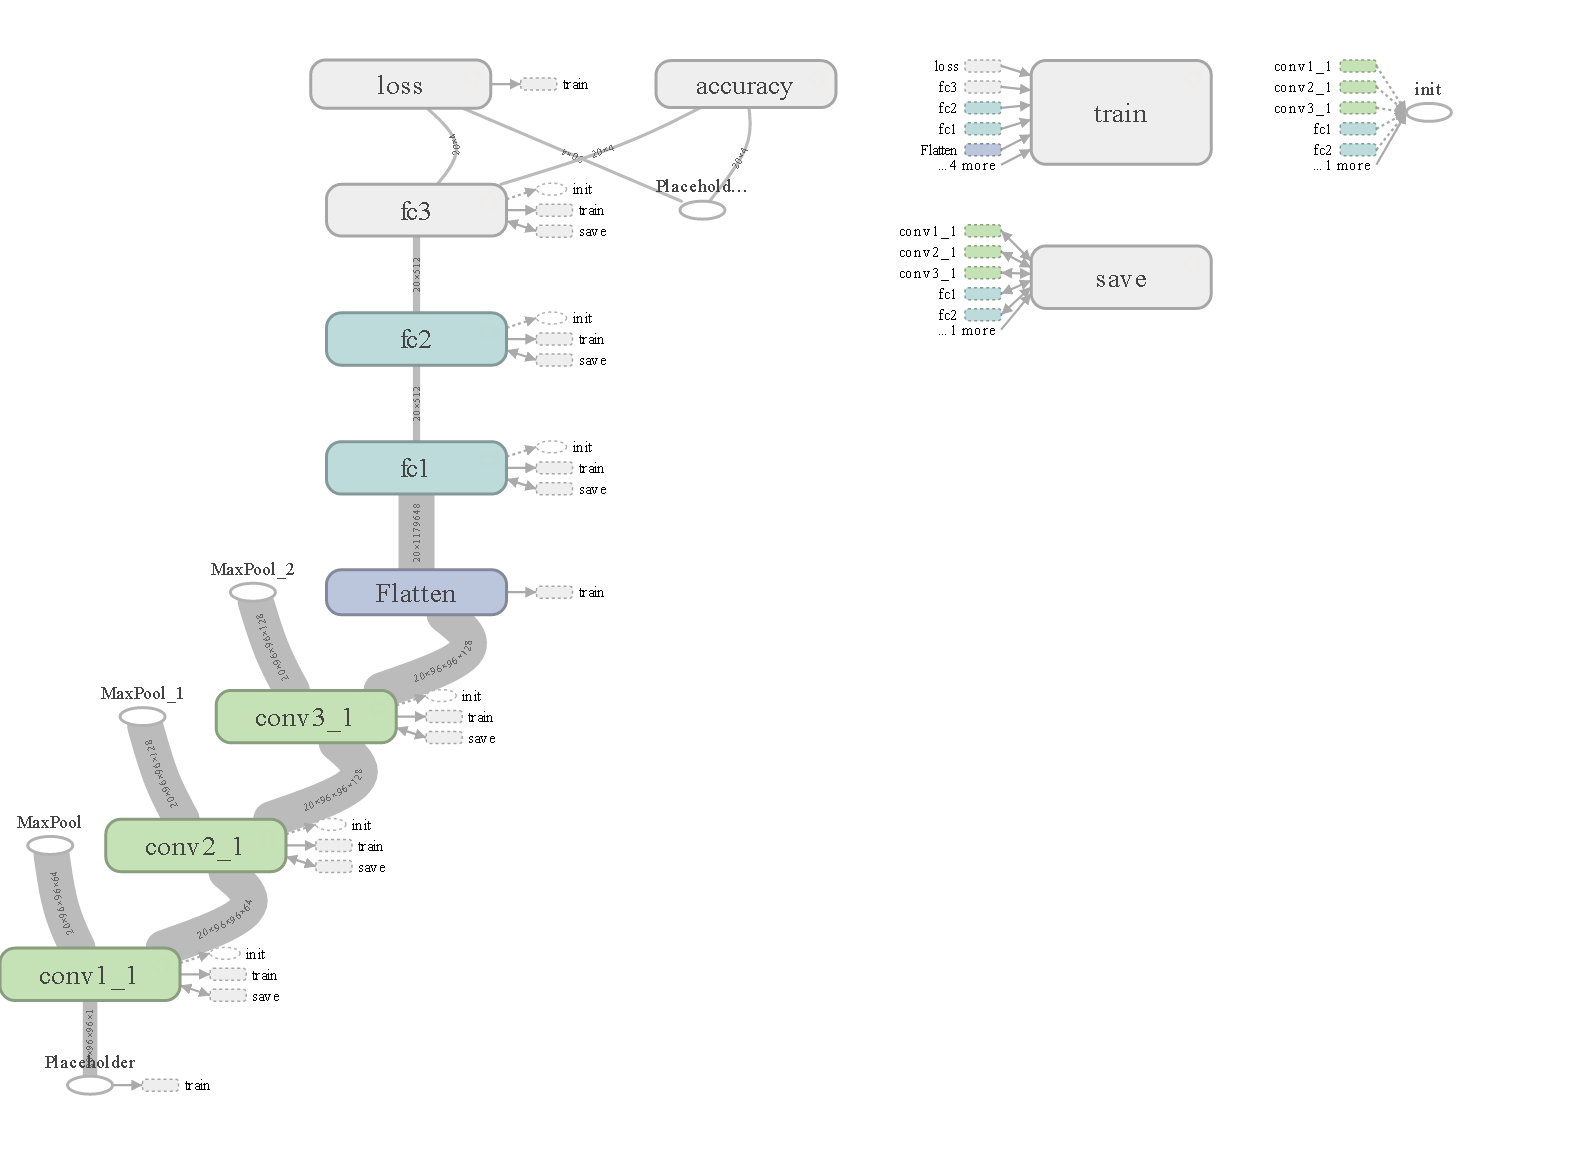
\includegraphics[scale=0.28]{images/graph-run.png}
	\caption{Aktueller Graphen des Beispiels}
	\label{fig:graphDig}
\end{figure}

\section{Verbesserungen}

Dieses Netzwerk stellt lediglich einen möglichen Lösungsansatz dar, mit welchem die Problemstellung verstanden werden soll. 
Im Grund existieren mehrere Möglichkeiten, um das Ergebnis des Netzwerks zu verbessern. 
Diese Möglichkeiten führen aber dazu, dass mehr Ressourcen benötigt werden. 
\begin{itemize}
	\item Verbreitern der Vollvernetzten-Ebenen, damit mehr Muster gespeichert werden können
	\item Convolutional-Ebenen doppelt ausführen 
	\item Grundanzahl an Convolutional-Ebenen erhöhen
	\item Anzahl der Datensätze durch Spiegeln verdoppeln
\end{itemize}






